% !TEX root = ../../my-thesis.tex

\graphicspath{{./content/conclusion/fig/}}

\chapter{Discussion}
\label{sec:conclusion}

\cleanchapterquote{To be but one with all living things, to return, by a radiant self-forgetfulness, to the All of Nature.}{Friedrich Hölderlin (1770-1843)}{}


Understanding ecological and economic systems involves the underpinning of general organizational principles at the origin of invariant patterns (\cite{Levin2002}, \cref{fig:forward_inverse_modelling}).
% 
Aiming at advancing our understanding of eco-evolutionary dynamics in ecological and economic systems, this thesis contributed to
% 
\begin{mylisti}
    \item a general understanding of the role of eco-evolutionary processes in shaping the dynamics of biological populations structured in complex landscapes (\cref{chap:diff-in-graphs}),
    \item the quantification of the effect of eco-evolutionary processes on the dynamics of economic systems at the country level (\cref{chap:econobiology}), and
    \item methodological advances in the forward and inverse modelling of eco-evolutionary dynamics (\cref{chap:diff-in-graphs,chap:mini-batching,chap:nonlocalPDE}).
\end{mylisti}
% 
In the following, I discuss the chapters of this thesis collectively, highlighting how they contribute to advance our current understanding of the dynamics of ecological and economic systems, and how they improve the current eco-evolutionary modelling paradigm. I further highlight current limitations, and propose future research directions.

\section{Contributions}

\subsection{Linking eco-evolutionary processes to patterns of differentiation}

Phenotypic differentiation arises from feedbacks between population dynamics, dispersal and mutations \citep{hamilton2021population}, and \cref{\chapi} determines how these feedbacks are modulated by landscape features.
% 
Mutations act upon individual organisms, and result in genetic drift in populations of finite size, causing stochastic variations in allelic proportions and phenotypes \citep{Slatkin1987a}. 
% 
In geographically structured populations, drift results in patterns of neutral differentiation \citep{Slatkin1987a}. 
% 
Migration fluxes reduce neutral differentiation by homogenizing differences in allelic proportions and phenotypes \citep{Slatkin1987a}, and this effect is further increased by landscape connectivity \citep{Wright1943,McRae2006,McRae2007} through the mechanism of "isolation by limited dispersal" \citep{Lande1991,Orsini2013}.
% 
When landscapes present heterogeneous habitats, natural selection can supplement the effect of genetic drift and increase the sole effect of stochasticity on differentiation \citep{fisher1958genetical}. Under this scenario, local environmental conditions select individuals with traits that provide them higher fitness \citep{Gaither2018}. At the population level, this results in populations adapting to their local environment, a mechanism coined "local adaptation" \citep{Kawecki2004} and resulting in patterns of "adaptive differentiation". 
% 
Adaptive differentiation is hindered by migration fluxes, which prevent local adaptation by destabilizing the evolution of traits towards the optimal \citep{Meszena1997,Debarre2013,Mirrahimi2020}.
% 
While adaptive differentiation concerns traits under selection, it indirectly affects the differentiation of neutral traits, that are co-evolving with traits under selection through linkages \citep{Billiard2015,Lepers2021}. This results in turn to the mechanism of "isolation by adaptation", where habitat heterogeneity, rather than landscape connectivity, increases neutral differentiation \citep{nosil2008}. 
% 
Simple mechanisms resulting in neutral and adaptive differentiation are identified, but how they are modulated by eco-evolutionary feedbacks and the topological features of realistic landscapes, presenting irregularities in connectivity \citep{Dale2010,LiebermanHauert2005}, is unclear. %TODO: unclear

In \cref{\chapi}, I demonstrate a novel mechanism, involving both the heterogeneity in connectivity of the landscape and the process of intra-specific competition, that considerably affects neutral differentiation. Through the creation of unbalanced migration fluxes, heterogeneity in connectivity increases the intensity of competition in highly connected populations. This, in turn, reduces gene flow and reinforces neutral differentiation.
% 
I also investigate the mechanism of local adaptation when habitat connectivity is irregular \citep{Dale2010,LiebermanHauert2005}. I show that the complexity of habitat spatial distribution can be reduced to a measure of habitat spatial auto-correlation, coined the "habitat assortativity". Landscapes characterized by a high habitat assortativity support populations that are systematically better adapted than in landscape with low assortativity. Specifically, I provide an analytical condition for local adaptation  (\cref{eq:m*}), that sheds light on how it relates to dispersal intensity, selection strength, habitat heterogneity, and habitat assortativity.

Because habitat assortativity affects local adaptation, it must also affect neutral differentiation through the mechanism of isolation by adaptation \citep{Orsini2013}. Closing the loop, I demonstrate that habitat assortativity affects neutral differentiation through two antagonistic effects. By favoring local adaptation, it promotes isolation by adaptation, therefore increasing neutral differentiation. In parallel, it favors gene flow within clusters of similar environmental conditions, decreasing isolation by limited dispersal. This results in habitat assortativity decreasing neutral differentiation for low dispersal intensity, and increasing neutral differentiation for high dispersal intensity (\cref{fig:setting2_4plots_M=7}).
% 
This complex feedback is essential to understand population differentiation in complex landscapes.
% 
\Cref{fig:summary_diff-in-graph} summarizes the feedback mechanisms underpinned in \cref{\chapi}. Overall, \cref{\chapi} establishes a comprehensive map of causal pathways involved in the phenotypic differentiation of populations structured in complex landscapes. 

\begin{figure}[t]
    \centering
    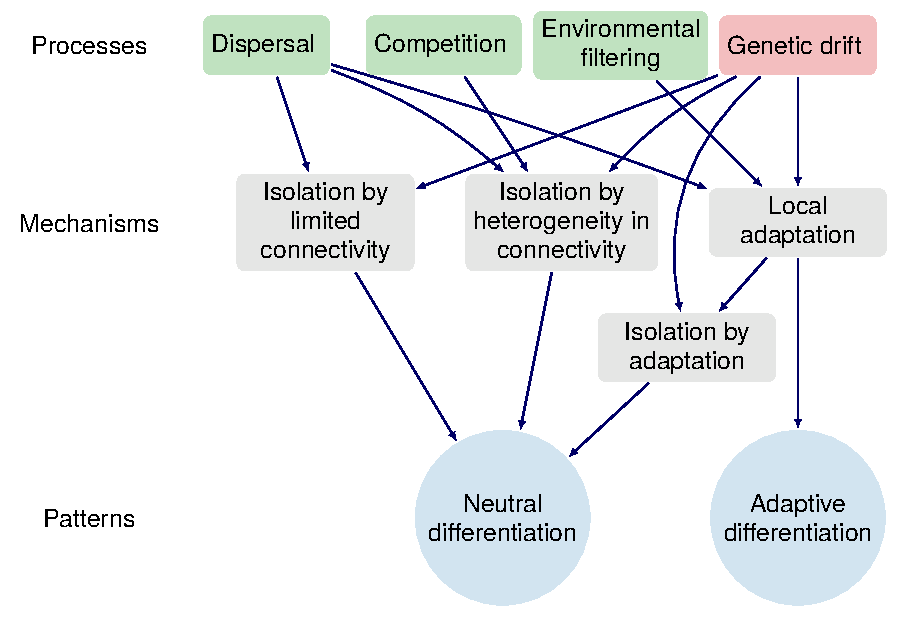
\includegraphics[width=\textwidth]{diff-in-graph.pdf}
    \caption{\textbf{Graphical representation of the eco-evolutionary mechanisms underpinned in \cref{\chapi} and involved in neutral and adaptive differentiation}. Ecological processes are displayed in green boxes, evolutionary processes are displayed in red boxes.}
    \label{fig:summary_diff-in-graph}
\end{figure}


\subsection{Linking economic patterns to eco-evolutionary processes}

Combining economic data and process-based models, \cref{\chapiii} bridges evolutionary economics, complexity economics and biology, advancing our general understanding of the forces driving the dynamics of economic systems.
% 
Evolutionary economics seeks to explain economic change with a forward modelling approach, using mechanistic models \citep{nelson1985evolutionary}.
% 
The processes of interactions between firms and economic activities, and evolutionary processes acting upon them, are the elemental forces accounted for \citep{Metcalfe2006}, but whether these eco-evolutionary processes can accurately characterize the long-run economic dynamics of countries remains to be demonstrated \citep{Hodgson2019}.
%Yet, evolutionary economics has up to now restricted its attention to subnational industrial dynamics \citep{Hodgson2019}.
% 
In contrast, complexity economics succeeds in predicting the economic dynamics of countries \citep{Hidalgo2021}, but is agnostic to the underlying processes \citep{Hidalgo2021}. Rather than using a forward modelling approach, it relies on world-wide economic data, processed with statistical techniques \citep{Mealy2019}, to measure differences in the structure of economic outputs across countries. The measurements are good predictors of economic growth \citep{Tacchella2018}, but a current concern is to unfold the causal processes \citep{Hidalgo2021}.

%%
Relying on inverse modelling, \cref{\chapiii} combines process-based models and data to deduct the main processes responsible for economic change.
% 
The approach undertaken relies on deep connections between processes acting upon economic activities and biological populations.
% 
Analogously to biological populations that are characterized by genes, economic activities are characterized by organizational routines \citep{nelson1985evolutionary}, which experience evolutionary processes and define how they engage in interactions with other economic activities \citep{nelson1985evolutionary}.
% 
As a result, economic activities can be considered as autonomous entities, which dynamics is determined by its characteristics and the processes acting upon them \citep{Boschma2005a}.
% 
The processes at stake leave characteristic signatures on the temporal dynamics of economic activities, consisting in distinctive temporal variations and couplings.
% 
These signatures can be identified with inverse modelling methods, estimating the support of population dynamic models embedding alternative hypothetical processes.

%%
\cref{\chapiii} tests whether the dynamics of economic activities at the national scale can be explained by positive and negative interactions between them, spatial dispersal processes, and/or economic transformations.
% 
Using population dynamic models capturing the different interdependencies, \cref{\chapiii} provides quantitative evidence that economic activities engage in positive interactions and disperse across countries.
% 
Positive interactions may arise from a variety of processes operating on firms, such as beneficial business interactions through supply chains \citep{Ozman2009,Saavedra2009a} and agglomeration externalities \citep{VanDerPanne2004}. 
% 
Its support implies that the dynamics of economic activities are highly inter-dependent, and suggests that diversity promotes economic development \citep{Hidalgo2018}.
% 
The spatial dispersal of economic activities may originate from the spatial diffusion of routines \citep{Hodgson2004} and knowledge spillovers \citep{Caragliu2016}. The discrepancies observed across countries in the strength-of-evidence for spatial dispersal suggest that economic activities are more akin to disperse in some countries than others. As an explanation, we propose that transfers of knowledge and routines may be blocked by barriers due to differences in cognitive, organizational, social, institutional or geographic proximity between countries \citep{Boschma2005,Caragliu2016}.
% 
\Cref{fig:summary_econobio} summarizes the ecological mechanisms evidenced in \cref{\chapiii}. Overall, \cref{\chapiii} provides quantitative evidences that, akin to biological systems, processes of interaction and dispersal shape the dynamics of economic systems at the country scale.

\begin{figure}[t]
    \centering
    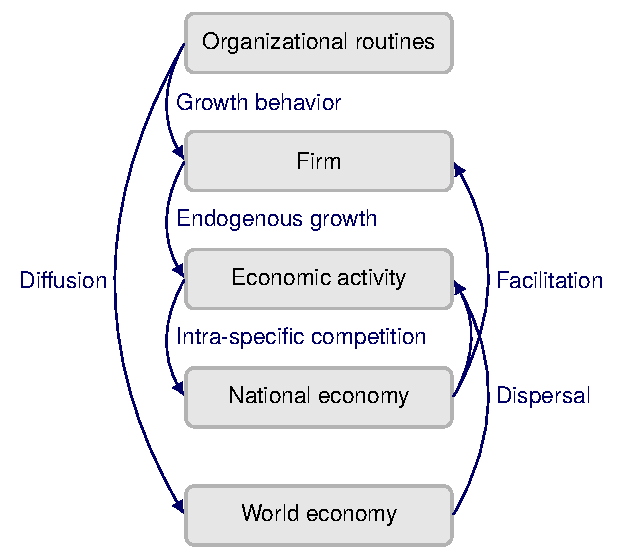
\includegraphics[]{econobio.pdf}
    \caption{\textbf{Graphical representation of the eco-evolutionary processes evidenced in \cref{\chapiv}, and how they affect the different organizational levels in economic systems.} \cref{\chapiv} provides quantitative evidences for the processes of mutualistic interactions (facilitation) and spatial dispersal, respectively coupling the world economy organizational level and the national economy organizational level, to the economic activity level. Directly depending on firms, the economic activity level is also coupled to the firm organizational level. Furthermore, in \cref{\chapiv}, we hypothesize that dispersal processes originate from the diffusion of organizational routines, coupling the organizational routines level to the world economy level.}
    \label{fig:summary_econobio}
\end{figure}

\subsection{Advances in the modelling of realistic spatial and phenotypic structures}

\Cref{\chapi,\chapiv} deliver new methods to incorporate important features of empirical systems within eco-evolutionary models.
% 
Evolutionary dynamics have traditionally been studied in the context of regular population structures \citep{LiebermanHauert2005}.
% 
For instance, to investigate differentiation in biological populations, a multitude of studies have considered regular spatial structures, missing the effect of spatial complexity on the underlying mechanisms \citep{Slatkin1973,Slatkin1978,Kirkpatrick1997,Polechova2015,Polechova2018,AndradeRestrepo2019,Doebeli2003,Meszena1997,Yeaman2011,Debarre2013,Mirrahimi2020}.
% 
Biological habitats differ in their connectivity \citep{Dale2010}, and economic entities are structured through complex networks \citep{Schweitzer2009}. \cite{LiebermanHauert2005} and subsequent studies of "evolutionary dynamics on graphs" (e.g., \cite{Tkadlec2019}) show that this complexity considerably affects the interplay between selection and drift. However, evolutionary dynamics on graphs does not consider eco-evolutionary feedbacks \citep{Govaert2019}.
% 
Thus far, models that capture eco-evolutionary feedbacks together with realistic, complex population structures were missing.

Another important feature of realistic biological populations that may affect their dynamics is the variety of traits that characterize them \citep{Doebeli2011}. While a vast majority of studies on eco-evolutionary feedbacks has focused on the evolution of scalar phenotypes \citep{Doebeli2011}, in most organisms, many phenotypic properties combine in complicated ways to determine ecological processes \citep{Doebeli2014}.
% 
For instance, \cite{Doebeli2011} shows that the consideration of multiple traits is likely to generate more phenotypic diversity than expected with one dimensional models.
% 
Trade-offs in traits are also essential features shaping the evolutionary dynamics of biological populations, with consequences on the dynamics of e.g. cancer cell evolution \citep{Fiandaca2021} and plankton dynamics \citep{LeGland2020}.
% 
Yet the simulation of eco-evolutionary models of biological populations structured over high dimensional phenotypic spaces is tremendously difficult, since the numerical cost of traditional simulation methods grows exponentially in the number of dimensions considered \citep{Bellman1957}. 

From first principles, \cref{\chapi} derives a stochastic individual-based model capturing eco-evolutionary feedbacks in populations structured in complex landscapes and high dimensional phenotypic space. \Cref{\chapiv} further provides tools to efficiently simulate a deterministic approximation of the individual-based model in high dimensional phenotypic spaces.
% 
The model presented in \cref{\chapi} involves the combination of graphs and high dimensional phenotypic spaces to model realistic population structures. Naturally capturing eco-evolutionary feedbacks, the model can readily be generalized to include other eco-evolutionary processes (see \cref{secSI:trait-dep-comp} for an extended variant with trait-based competition). The Julia library \textbf{Evoid.jl}, that I have written for the purpose of the numerical experiments in \cref{\chapi} and that is publicly available \citep{Evoid}, already implements a generic version of the model. %(), 
% 
As such, the model presented in \cref{\chapi} and the Julia library \textbf{Evoid.jl} may be used to investigate other questions involving complex population structures \citep{LiebermanHauert2005} and the co-evolution of characteristics \citep{Doebeli2011}.
% 
While they can realistically reproduce the discrete and stochastic nature of ecological and evolutionary processes \citep{deangelis2005individual}, numerical simulations of individual-based model may not provide a general understanding of system investigated \citep{Lion2016,Hodgson2019}, and cannot be scaled to simulate large systems involving a large number of individuals \citep{deangelis2005individual}. Yet, the individual-based model proposed in \cref{\chapi} is mathematically tractable, and can be approximated with a deterministic PDE approximation under simplifying assumptions.
% 
The mathematical tractability allows obtaining analytical insights on how the interplay between the processes acting upon the individuals transform into mechanisms affecting the population level (\cref{\chapi}).
% 
The PDE approximation, combined with the numerical methods presented in \cref{\chapiv}, further allow efficient simulations. 
% 
The numerical methods proposed in \cref{\chapiv} are now implemented in a new registered Julia package that I have released under the name of \textbf{HighDimPDE.jl} \citep{HighDimPDE}, now belonging to the SciML organisation \citep{Rackauckas2020a}.
%
The package aims at hosting many more solver algorithms that can efficiently simulate high dimensional PDEs, and has, as of September 2022, already received contributions from 5 independent developers (see \cite{contribHighDimPDE}). These contributions may greatly enhance \textbf{HighDimPDE.jl} over the years, promising efficient simulations of eco-evolutionary models.
% 
Together, \cref{\chapi,\chapiv} deliver novel tools to advance our understanding of the effect of the complexity of spatial and phenotypic structures on eco-evolutionary dynamics.


\subsection{Advances in inverse modelling for identifying eco-evolutionary processes in empirical systems}

Our understanding and prediction of eco-evolutionary dynamics in ecological and economic systems critically depends on the confrontation of process-based models with empirical data \citep{Pelletier2009,Hidalgo2021}.
% 
The most celebrated inference methods for inverse modelling in biology are Bayesian inference methods with Markov Chain Monte Carlo \citep{Lignell2013,Higgins2010,Xu2006,Fiechter2013,Rosenbaum2019} and variational methods \citep{Schartau2017}.
% 
Bayesian inference methods require numerous forward model integrations \citep{Schneider2017}, and are highly affected by the number of model parameters \citep{Csillery2010}.
% 
Variational methods require the model sensitivity to its parameters \citep{Schartau2017} and are prone to converge to local minima, especially with complex models \citep{Gabor2015}.
% 
Those central issues likely explain the very limited use of inverse modelling to further our knowledge on eco-evolutionary processes in ecological systems (but see \cite{Sukumaran2016,Skeels2019,Skeels2022} that use approximate Bayesian computation methods). 

%
%% Our method
\cref{\chapii} presents a novel inverse modelling framework that allows to estimate the parameter values and the support of complex eco-evolutionary models from temporal data.
% 
The framework is based on a variational method, but resolves its main shortcomings by heavily relying on automatic differentiation \citep{Rackauckas2020a}, state-of-the-art optimizers \citep{Kingma2014}, and a learning strategy based on a segmentation method. 
% 
The use of automatic differentiation simply eliminates the effort required to obtain the model sensitivity to its parameters, and the state-of-the-art optimizers, together with the segmentation method, ensure the efficiency and robustness of the method in handling highly nonlinear models.
% 
\cref{\chapii} takes part in an ongoing effort to blend machine learning (ML) and traditional models to gain scientific understanding and extrapolability \citep{Karpatne2017,Rackauckas2020a,Schneider2017,Rolnick2023,Kashinath2021,Yazdani2020,Raissi2019}. 
% 
In physical systems such as oceanic and atmospheric systems, general organizational principles are known and formulated in general circulation models, where ML is mostly used to accelerate simulations \citep{Kashinath2021} and improve model forecast skill \citep{Schneider2017}. In contrast, general models of ecological and economic systems are yet to be formulated, and methods such as the ML framework presented in \cref{\chapii} can greatly contribute to identifying the general organizational principles required to reach this goal \citep{Karpatne2017}. 
% 
By contrasting competing hypotheses embedded in alternative models, \cref{\chapii,\chapiv} provide concrete examples, both with synthetic and empirical data, that the inverse modelling framework in \cref{\chapii} can successfully elucidate eco-evolutionary mechanisms.
%% 
Integrating the practical constraints of current ecological datasets \citep{Dornelas2018}, the inverse modelling framework may also be relevant for improving the forecast ability of existing eco-evolutionary model \citep{Norberg2012}.
% 
Built thanks to the composability of the celebrated differential equation solver \textbf{DifferentialEquations.jl} and the deep learning library \textbf{Flux.jl}, the inverse modelling framework is implemented in a new, multipurpose Julia package readily available to the scientific community, that I have released under the name of \textbf{PiecewiseInference.jl} \citep{PiecewiseInference}.
% 
Together, the inverse modelling framework proposed in \cref{\chapii} successfully blends ML methods with mechanistic ecosystem models to gain scientific knowledge from observation data. 

\section{Limitations}
\label{sec:limitations}
\subsection{Computational complexity for modelling the evolution of full phenotypic densities}
Alternative methods to those presented in \cref{\chapi,\chapiv} may be more appropriate for the forward modelling of eco-evolutionary dynamics.
% 
While individual-based models are interesting tools to investigate stochastic drift in finite size populations, the Gillespie algorithm \citep{Gillespie1976} employed to simulate the individual-based model in \cref{\chapi} is computationally intensive, and requires to compute the fitness of all individuals at each birth or death event, which depends on the characteristics of all the other individuals. The resulting computational complexity scales poorly with the number of individuals involved, preventing its use to model large populations. 
% 
PDE approximations are computationally more efficient in large populations for low dimensional phenotypic spaces ($\lessapprox 3$-dimensional). 
% 
% The computational complexity of standard approximation methods grows exponentially in the number of dimensions of the phenotypic space, but 
% 
The methods presented in \cref{\chapiv} can efficiently simulate PDE models in higher dimensions (demonstrated up to 10 traits), but still suffer from a number of issues that may prevent their practical use.
% 
First, the MLP method can only provide the population number for one single trait value in one run. Consequently, the MLP method cannot characterize the total population density with a reasonable computational complexity. 
% 
In contrast, the full population density can be obtained with the ML-based approximation method, but the method involves the training of many neural networks (one at each time step). This is worrying, since long time horizons are required by practitioners, and that the training of a neural network is numerically costly. Another problem with the numerical methods proposed in \cref{\chapiv} is that they involve the tuning of meta parameters, including the choice of a measure for the integration of the non-local term ($\nu_x$ in \cref{frame:mlpsetting,def:general_algorithm}). Though this choice is critical to the success of the numerical simulations, it is unclear how it can be determined.
% 
While greatly decreasing the computational cost of traditional methods, the novel methods proposed in \cref{\chapiv} are still computationally demanding and require a delicate tuning of the meta-parameters. 

Because PDE models track the evolution of the full phenotypic density of populations, PDE models inevitably require a considerable computational effort -- irrespective of the numerical method used. 
% 
Nevertheless, only the first three moments of the population density are usually of interest, namely population size, trait mean and trait variance \citep{Nordbotten2020}. 
% 
Instead of seeking to numerically approximate the full phenotypic density, moment closure approximation methods \citep{Wickman2021,Lion2022,Nordbotten2020} may instead be considered. Those approaches consist in approximating the population density with a multivariate Gaussian distribution. This, in turn, allows to transform the PDE problem into a system of coupled differential equations involving the time evolution of the population size (1 variable for a single species population), the mean trait values ($d$ scalar variables), and the variance-covariance matrix of the multidimensional trait density ($d^2$ variables). As such, the computational cost of this method only scales polynomially with the number of dimension ($\mathcal{O}(d^2)$), while providing the sufficient information required to investigate eco-evolutionary dynamics in high dimensional phenotypic spaces. 
% 
It is worth noting that instead of using neural networks, multivariate Gaussian functions could also be used within the ML-based method for simulating eco-evolutionary models. Equivalent to the simplifying assumption taken with moment closure methods, we expect this approach to greatly improve the computational efficiency of the ML-based method, as they involve fewer free parameters ($d(d+1) + 1$, i.e. 111 parameters for $d=10$) than neural networks ($(d+50)(2d+50) + 3(d+50) + 1$ parameters used for the examples in \cref{subsec:fisherKPP_neumann_r,subsec:nonlocalcompPDE,subsec:sinegordon_nonlocal,subsec:aniso_mutator_selector,subsec:allen_cahn}, i.e. 4381 parameters for $d=10$).
% while solving the problem of the choice of $\nu_x$. 
In summary, using the ML-based approximation presented in \cref{\chapiv} with multivariate Gaussian functions may considerably lower the number of iterations required in the training process, while reducing the computational cost.

The proposed methods in \cref{\chapi,\chapiv} suffer from considerable computational cost, because they seek to simulate PDE models which track the evolution of the full phenotypic distribution of populations. Because only the population number, the mean and the variance-covariance matrix of the phenotypic distributions are of interest, closure approximation methods could be considered. Those methods are compatible with the ML-based method proposed in \cref{\chapiv}.


\subsection{Uncertainty estimation and model selection bias}
The inverse modelling framework proposed in \cref{\chapii} and used in \cref{\chapiii} also presents pitfalls.
%
First, the mini-batching learning strategy requires the choice of a segmentation size to ensure the convergence to the maximum likelihood estimate. This choice should be motivated by the roughness of the model likelihood landscape (see \cref{subsec:minibatch_implementation}), but may affect the model selection process:
% 
a small batch size implies that the model goodness-of-fit is evaluated on the fast dynamics of the data, while the resulting support could differ, were the model fitted with a higher segmentation size. Theoretical developments are required to provide statistically justified guidance for the choice of the segmentation size. 
% 
Second, the maximum likelihood estimate of models with complex likelihood landscape may be underestimated, because not correctly identified. As a result, the model selection process may be biased towards models which associated likelihood landscape is easier to navigate. 
% 
Third, the information criterion-based model selection procedure used in \cref{\chapii,\chapiii} is uniquely based on a trade-off between the goodness-of-fit and the number of parameters of the model, which may not be satisfactory to characterize process-based models \citep{Clermont2015}. 
% 
Other criterion, for instance based on the complexity of the dynamical behavior of the model (such as, e.g., its Lyapunov exponent), could be developed.
% 
Fourth, the inverse modelling framework developed in \cref{\chapii} requires a differentiable model, a strong prerequisite that may not be met by, e.g. stochastic models. 
% 
Fifth, the inverse modelling framework only provides the maximum of the posterior distribution, while the posterior distribution may be multimodal, with alternative modes carrying valuable information \citep{Wilson2020}.%, and in this case, the consideration of the full posterior distribution, obtained with fully Bayesian methods, may be more appropriate for model selection.

% 
Alternatively, \cite{Sukumaran2016,Skeels2019,Skeels2022} employ variants of approximate Bayesian computation methods \citep{Csillery2010} for eco-evolutionary model selection. Their approach consists in aggregating model simulation outputs into summary statistics, used to train classifier algorithms (such as, e.g., random forests or neural networks) in recognizing the signatures of the competing models. Once trained, the classifier algorithms are used on the summary statistics obtained from the empirical data, discriminating between the alternative hypotheses. 
% 
This approach does not require model differentiability, and is consequently more flexible than the method proposed in \cref{\chapii}. Also, the use of summary statistics can elucidate which particular feature of the empirical data is better explained by a given model. 
% 
Nevertheless, this strength is a pitfall: summary statistics necessarily reduce the information contained in empirical data, which can prevent to correctly discriminate between models \citep{Csillery2010}.
% 
Altogether, the segmentation inverse modelling framework in \cref{\chapii} is sensitive to the segmentation size, requires models to be differentiable, and does not provide uncertainty estimation. While approximate Bayesian computation may be a valuable alternative, it also presents restrictive shortcomings. Still, the segmentation learning strategy extends beyond the framework proposed, and could be used in combination with novel approaches in Bayesian computation to combine the best of both worlds.

\section{Perspectives}

\subsection{Development opportunities in inverse modelling}

The segmentation method presented in \cref{\chapii} and the ML-based approximation method developed in \cref{\chapiv} offer unique development opportunities to leverage inverse modelling.
%
The segmentation method is relevant beyond the ML framework presented in \cref{\chapii}, and could be used within a fully Bayesian framework, where the full posterior distribution of the model is estimated. Compared to considering a standard formulation of the likelihood function such as in \cref{eq:likelihood-std}, using the segmentation loglikelihood formulation proposed in \cref{eq:ML-framework} results in a smoother posterior distribution, which should reduce the large number of forward model integration required by Bayesian inference.
% 
While this number could still be prohibitively expensive for Bayesian inference with MCMC chains, automatic differentiation variational inference (ADVI, \cite{Morningstar2020,Gosh2021}) offers an appealing alternative. In ADVI, the posterior distribution is approximated by a Gaussian distribution \citep{Morningstar2020}, significantly reducing the number of model integration \citep{Morningstar2020}. Improving the ML framework presented in \cref{\chapii}, ADVI could capture multimodality in the model posterior distribution (by approximating the multimodal distribution with a gaussian distribution with large variance). This, in turn, could improve the robustness of model selection (\cref{sec:limitations}), and provide uncertainties estimations on the parameters.
% 
Bayesian Learning via Stochastic Gradient Langevin Dynamics \citep{Welling2011BayesianLV} is an alternate solution to ADVI, that could readily be used with the ML framework proposed in \cref{\chapii} instead of the optimization algorithms suggested. This algorithm builds upon recent advances in Bayesian deep learning \citep{Wilson2020}, and interprets the iterative gradient-based optimization procedure as a Markov chain with an equilibrium distribution over the posterior distribution of the model parameters. It therefore comes with the scalability of variational methods and the interpretability of Bayesian methods, providing uncertainty estimates while ensuring computational efficiency.


%%
For inverse modelling with PDE models, an extension of the ML-based approximation method presented in \cref{\chapiv} could yield interesting performance.
% 
In \cref{def:general_algorithm}, the parameters of the PDE model are assumed fixed, but could be set as free parameters, analogously to the parameters of the neural networks used for approximating the PDE solution. The loss function in \cref{eq:loss_general_case} would then take the PDE model parameters as additional arguments, and include an additional term, penalizing the distance between the PDE model solution and the data. This term, analogous to \cref{eq:ML-framework} in \cref{\chapii}, would constrain the PDE parameters, similarly to the training of physics informed neural networks \citep{Raissi2019,Yazdani2020}.
% 
Yet in contrast to \cite{Raissi2019,Yazdani2020}, a major advantage of this approach is to efficiently perform inverse modelling with high-dimensional dynamical models. Because Julia is a programming language with pervasive automatic differentiation (see \cref{subsec:Julia} in \cref{chap:intro}), this development would require little effort with the Julia library \textbf{HighDimPDE.jl}.
% 
Altogether, the ML methods developed in \cref{\chapii,\chapiv} offer unique opportunities to grant more robustness and efficiency to inverse modelling methods, providing uncertainty estimation and the possibility to handle high dimensional models.


\subsection{Confronting eco-evolutionary model on spatial graphs and empirical data}

The confrontation of the predictions obtained in \cref{\chapi} with empirical data, and the use of empirical data to constrain the eco-evolutionary model on spatial graphs presented in \cref{\chapi}, could advance our understanding of eco-evolutionary dynamics in empirical systems.
% 
In \cref{\chapi}, we predicted three topology metrics to correlate with standard population differentiation metrics ($Q_{ST}$ metrics). By projecting real landscapes on spatial graphs (see \cite{Dale2010} and \cref{figSI:graph_real_land}), the topology metrics, together with empirical data on population differentiation, could be used to verify our predictions. Discrepancies may indicate that additional processes are involved in population differentiation in empirical systems. On the other hand, a validation of the predictions from \cref{\chapi} could help to predict population differentiation at a global scale. These predictions could, in turn, be linked to patterns of species richness, in order to underpin how population differentiation may lead to speciation over time \citep{Templeton1981}.

Hindcasts with the eco-evolutionary model on spatial graphs over geological time, using paleo-climatic data \citep{STRAUME2020126} as environmental condition forcings, could also help to address fundamental questions on the processes involved in spatial biodiversity patterns. In contrast to deep-time spatially explicit eco-evolutionary models (see \cite{Hagen2022} for a review), the model developed in \cref{\chapi} does not assume a timescale separation between ecological and evolutionary processes.
% 
This would allow disentangling, for instance, the role of feedbacks between trait-based competition \citep{Dieckmann1999} -- succinctly considered in \cref{\chapi} (see \cref{secSI:trait-dep-comp}) --, and environmental filtering \citep{Doebeli2003}, in shaping patterns of species distribution \citep{Rahbek2019a}.

Along shorter time scales, the eco-evolutionary model on spatial graph could be calibrated on empirical data of species distribution (see, e.g., \cite{Abegg2020,GBIF:TheGlobalBiodiversityInformationFacility2022}) with the inverse modelling method proposed in \cref{\chapii}, to better predict how biological populations will adapt to climate change \citep{Norberg2012,Urban2016}. Using climate projections \citep{Kriticos2012} as environmental forcings, the model could capture the processes of spatial dispersal and adaptation, that are fundamental yet neglected in models currently used for biodiversity forecasts \citep{Pearson2003}.
% 
Last but not least, multiple species or functional groups could also be accounted for in the model proposed in \cref{\chapi}. Tracking suitable environmental conditions, species ranges are expected to shift towards higher elevations and higher latitudes \citep{Chen2011}, but how this will modify trophic interactions and ecosystem dynamics is unclear \citep{Descombes2020}.
% 
The model would provide a framework to explore how global warming may generate feedbacks between the processes of dispersal, species' evolutionary response, and trophic interactions, collectively affecting ecosystem dynamics.
% 
In summary, confronting the predictions of \cref{\chapi} with empirical data, extensions of the model developed in \cref{\chapi}, together with the use of the ML framework presented in \cref{\chapii}, could bring further insights on the actual mechanisms involved in empirical systems, and help to predict their responses to climate change. 


\subsection{Econobiology, a new venue to understanding economic systems, and designing more appropriate governance}

The success of the biologically inspired model presented in \cref{\chapiii}  in characterizing the dynamics of economic activities calls for a deeper investigation of commonalities and differences in organizational principles in ecological and economic systems.
% 
As a first step, I suggest investigating whether the results of \cref{\chapiii} hold for finer levels of economic activity aggregation, as more detailed data on economic activities is available \citep{Hausmann2011}. 
% 
Second, the eco-evolutionary models should be complexified, to investigate whether it can capture more detailed aspects of the dynamics (see \cref{sec:discussion-econobio} in \cref{\chapiii}).
% 
In parallel, a promising research direction is to better understand how capital fluxes \citep{King1993} compare with fluxes of matter and energy \citep{Veldhuis2018} in ecological systems.
% 
\cite{Veldhuis2018} provides an excellent synthesis of our understanding of how ecosystem organization emerges through self-reinforcing eco-evolutionary mechanisms. This synthesis is an interesting roadmap to formulate hypotheses and investigate analogous self-reinforcing mechanisms determining fluxes of capital in economic systems. 
% 
There may be deep connections between nutrient cycles and capital cycles, where ecological compartments and financial intermediaries develop to improve the efficiency of nutrient flows and capital allocations \citep{Odum1969}.
% 
\cite{Veldhuis2018,King1993} show that, in both ecological and economic systems, this efficiency sustains productivity and growth, but that the developmental process may fail. In the latter case, ecosystems may stay in a state of lower maturity \citep{Margalef1963} and economies may be stuck in a technological lock-in \citep{C.A.HidalgoB.Klinger}. 
% 
I expect that this research venue will pinpoint key organizational differences between ecological and economic systems. Since they have undergone evolution for a much longer time than economic systems, ecological systems may be more effective and resilient than economic systems, providing guidance for economic policies.
% 
Together, future directions should seek to understand similarities and differences in organizational principles in ecological and economic systems, which may eventually help improving economic regulations.


\section{Concluding remarks}


Bridging biology, mathematical modelling, machine learning and economics, this thesis advances our general understanding of eco-evolutionary processes and feedbacks in ecological and economic systems. It also provides novel modelling tools, that were publicly released in Julia packages to join efforts and collectively advance this understanding.
% 
While we now better understand eco-evolutionary feedbacks in spatially structured populations, we are still far from a general understanding of their role at the ecosystem level. 
% 
The challenge is enormous, because anthropogenic pressure and climate change are rapidly affecting ecosystems.
% 
Methods similar to those presented in this thesis, combining machine learning and process-based models, can massively accelerate the underpinning of general principles at the ecosystem level, and provide reliable forecasts. This, in turn, should help designing adequate management of ecosystem services to mitigate the consequences of human development.
% 
Machine learning, together with evolutionary biology, can also help us to underpin general principles in economic systems. Paving the way, this thesis demonstrates that analogous processes to those shaping ecosystems have major effects on economic change. Future research will tell whether economic and ecological systems have deeper organizational principles in common.
% 
Realizing overlaps and differences can help us to design better economic policies. 
% 
Our young economic systems can surely learn from ecological systems, that have survived major crises for more than 3.5 billion years.
% 
Philosophically speaking, this realization invites us to demonstrate more humility towards ecological systems, and "\textit{[...] to return, by a radiant self-forgetfulness, to the All of Nature}".